\begin{lemma}
    \label{lemma::arcsin-over-pi-has-OEX}
        Let $f(x) = \sin(\pi x)$ and $I=(a,b)$ with $a,b\in \Rationals$ and $-1<a<b<1$. Then there is an effective open exhaustion for $f^{-1}(I)$.
    \end{lemma}
    \begin{proof}
        Let us consider $f^{-1}(x) = \arcsin(x)/\pi$. The function $f^{-1}$ is clearly \WhileCC-approximable.
        We know that
        \begin{itemize}
            \item The function $f^{-1}$ is monotonically increasing.
            \item The function $f^{-1}$ is defined on $(a,b)$.
        \end{itemize}
        Hence, Theorem \ref{thm::OEX_by_WCC_approximability} gives us an open exhaustion for $f^{-1}(I)$, and this completes the proof.
    \end{proof}
    \begin{theorem}
    \label{thm::OEX_sin}
       The function $\sin(x)$ is \effectivelyOpen{}. 
    \end{theorem}
    \begin{proof}
        It suffices to show that $f(x)=\sin(\pi x)$ is \effectivelyOpen{}.
        Using Remark \ref{remark::OEX_for_interval_implies_OEX_for_all_open_sets}, we only need to prove that $f^{-1}(I)$, if nonempty, has an effective open exhaustion for any $I=(a,b)$ with $a<b \in \Rationals$. Let us consider the value of $a$ and $b$: 
        \begin{itemize}
            \item $-1<a<1<b$:
                In this case we can use Theorem \ref{remark::OEX_for_interval_implies_OEX_for_all_open_sets} along with Lemma \ref{lemma::arcsin-over-pi-has-OEX}, we can get an open exhaustion for $f^{-1}((a,1/2))$. We modify each $(a_i, b_i)$ to 
                \begin{center}
                    $(a_i-2i, -1-a_i-2i)\cup \cdots \cup (a_i-2, -1-a_i-2)$\\
                    ${}\cup(a_i, -1-a_i)$\\
                    ${}\cup (a_i+2, -1-a_i+2) \cdots (a_i+2i, -1-a_i+2i)$
                \end{center}
                Note that the reason we are modifying each interval is that the open exhaustion $f^{-1}((a,1/2))$ does not cover $x=1/2$, so stretching $(a_i, b_i)$ to $(a_i, 1- a_i)$ will help cover the point $x = 1/2$ as well as the mirrored interval $(1/2, 1-f(a))$.
                \begin{figure}[H]
    \centering
    \caption{Covering the points with $f(x) = 1$}
    \label{fig::sin-explanation}
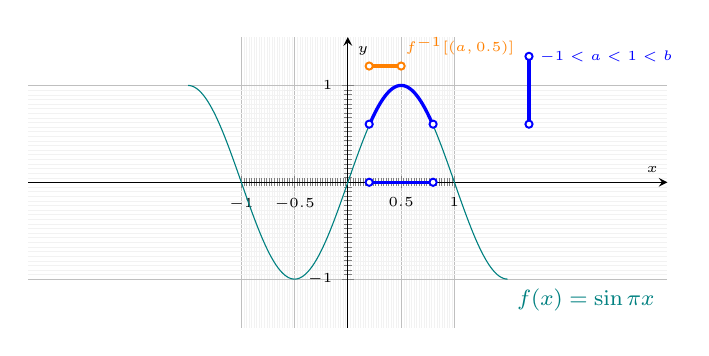
\begin{tikzpicture}
    \begin{axis}[
        width = 0.8\textwidth,
        grid=both,
        minor tick num=20,
        grid style={line width=.1pt, draw=gray!10},
        major grid style={line width=.1pt,draw=gray!50},
        axis lines=middle,clip=false,
        height = 150,
        xmin=-3,xmax=3,ymin=-1.5,ymax=1.5,
        ytick={-1,0,1},
        xtick={-1,-0.5,0,0.5,1},
        font=\tiny,
        xticklabels={$-1$,$-0.5$,$0$,$0.5$,$1$},
        xticklabel style={black},
        xlabel=$x$,
        ylabel=$y$
    ]
    \draw[very thick, blue] (axis cs:1.7,0.6) -- (axis cs:1.7,1.3) node[right, font=\tiny] {$-1<a<1<b$};
    \fill [color=white,draw=blue,line width=0.7pt] (axis cs:1.7,0.6) circle (1.3pt);
    \fill [color=white,draw=blue,line width=0.7pt] (axis cs:1.7,1.3) circle (1.3pt);

    \addplot[domain=-1.5:1.5,samples=150,teal]{sin(deg(pi*x))}
                                node[below right,pos=1,font=\footnotesize]{$f(x)=\sin \pi x$};

    \addplot[domain=.2:0.8,samples=100, very thick,blue]
        {sin(deg(pi*x))} node[below right,pos=1,font=\footnotesize]{};
    \addplot[domain=.2:0.8,samples=100, very thick,blue]
        {0} node[below right,pos=1,font=\footnotesize]{};

    \fill [color=white,draw=blue,line width=0.7pt] (axis cs:0.2,0.6) circle (1.3pt);
    \fill [color=white,draw=blue,line width=0.7pt] (axis cs:0.8,0.6) circle (1.3pt);

    \fill [color=white,draw=blue,line width=0.7pt] (axis cs:0.2,0) circle (1.3pt);
    \fill [color=white,draw=blue,line width=0.7pt] (axis cs:0.8,0) circle (1.3pt);
    
    \addplot[domain=.2:0.5,samples=100, very thick, orange]
        {1.2} node[above right,pos=0.8,font=\tiny]{$f^{-1}[(a,0.5)]$};
    \fill [color=white,draw=orange,line width=0.7pt] (axis cs:0.2,1.2) circle (1.3pt);
    \fill [color=white,draw=orange,line width=0.7pt] (axis cs:0.5,1.2) circle (1.3pt);
    \end{axis}
  \end{tikzpicture}
\end{figure}

                The reason we are adding $(a_i-2i, -1-a_i-2i)\cup \cdots \cup (a_i-2, -1-a_i-2)$ and $(a_i+2, -1-a_i+2) \cdots (a_i+2i, -1-a_i+2i)$ is that $f(x)$ is a periodic function and we would want to eventually cover all the $x$s in $\Reals$ for which $f(x)$ falls in $(a,1]$.
                The intuition for building up the stages is shown in Figure \ref{fig::sin-explanation}.
                \begin{figure}
    \centering
    \caption{Visualization of our algorithm for building up stages for the preimage of an interval $(a,b)$ with $-1<a<1<b$}
    \label{fig:sin-a1b-step1}

    \begin{subfigure}{\textwidth}
        \centering
        \caption{stage 0}
        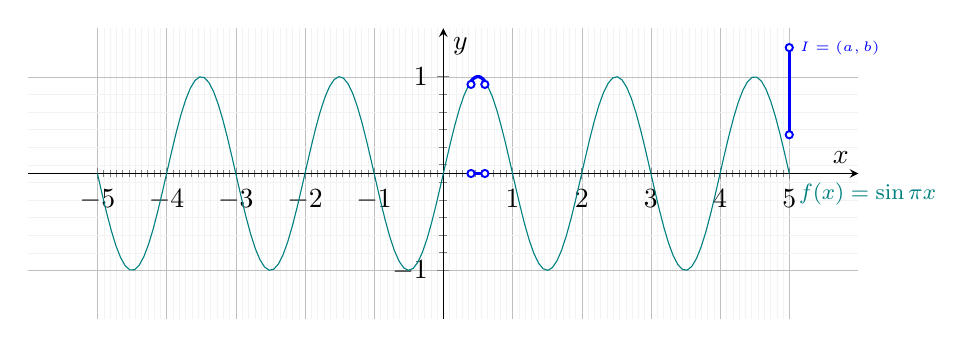
\begin{tikzpicture}
    \begin{axis}[
        width = \textwidth,
        grid=both,
        minor tick num=10,
        grid style={line width=.1pt, draw=gray!10},
        major grid style={line width=.1pt,draw=gray!50},
        axis lines=middle,clip=false,
        height = 150,
        xmin=-6,xmax=6,ymin=-1.5,ymax=1.5,
        ytick={-1,1},
        xtick={-5,-4,-3,-2,-1,0,1,2,3,4,5},
        xticklabels={$-5$,$-4$, $-3$,$-2$,$-1$,$0$,$1$,$2$,$3$, $4$, $5$},
        xticklabel style={black},
        xlabel=$x$,
        ylabel=$y$
    ]
    \draw[very thick, blue] (axis cs:5,0.4) -- (axis cs:5,1.3) node[right, font=\tiny] {$I=(a,b)$};
    \fill [color=white,draw=blue,line width=0.7pt] (axis cs:5,0.4) circle (1.3pt);
    \fill [color=white,draw=blue,line width=0.7pt] (axis cs:5,1.3) circle (1.3pt);


    \addplot[domain=-5:5,samples=150,teal]{sin(deg(pi*x))} node[below right,pos=1,font=\footnotesize]{$f(x)=\sin \pi x$};

    \addplot[domain=.4:0.6,samples=100, very thick,blue]
    {0} node[below right,pos=1,font=\footnotesize]{};
    
    \addplot[domain=.4:0.6,samples=100, very thick,blue]
        {sin(deg(pi*x))} node[below right,pos=1,font=\footnotesize]{};
    \fill[color=white,draw=blue,line width=0.7pt] (axis cs:0.4,0.92) circle (1.3pt);
    \fill[color=white,draw=blue,line width=0.7pt] (axis cs:0.6,0.92) circle (1.3pt);
    \fill[color=white,draw=blue,line width=0.7pt] (axis cs:0.6,0) circle (1.3pt);
    \fill[color=white,draw=blue,line width=0.7pt] (axis cs:0.4  ,0) circle (1.3pt);

    \end{axis}
  \end{tikzpicture}
    \end{subfigure}
    \begin{subfigure}{\textwidth}
        \centering
        \caption{stage 1}
        \input{images/4/sin-a1b-step2}
    \end{subfigure}
    \begin{subfigure}{\textwidth}
        \centering
        \caption{stage 2}
        \input{images/4/sin-a1b-step3}
    \end{subfigure}

\end{figure}
            \item $-1<a<b<1$:
                In this case we can use Theorem \ref{remark::OEX_for_interval_implies_OEX_for_all_open_sets} we can get an open exhaustion for $f^{-1}(I)$. For each stage we modify each $(a_i, b_i)$ to 
                \begin{center}
                    $(a_i - 2i, b_i-2i) \cup \cdots \cup (a_i, b_i) \cup \cdots \cup (a_i+2i, b_i+2i)$
                \end{center}
            \item $a,b >1$ or $a,b<-1$: In this case $f^{-1}(I) = \emptyset$.
            \item $a<-1<b<1$:
                In this case we can use Theorem \ref{remark::OEX_for_interval_implies_OEX_for_all_open_sets} we can get an open exhaustion for $f^{-1}\paren{(-1/2,b)}$. We modify each $(a_i, b_i)$ to 
                \begin{center}
                    $(-1-b_i-2i, b_i-2i)\cup \cdots \cup (-1-b_i-2, b_i-2)$\\
                    $\cup(-1-b_i, b_i)$\\
                    $\cup (-1-b_i+2, b_i+2) \cdots (-1-b_i+2i, b_i+2i)$
                \end{center}
                
            \item $a<-1<1<b$: In this case the open exhaustion is 
                \[
                ((-1, 1), \ldots, (-k-1, k+1), \ldots).
                \]
                This gives us an effective open exhaustion for $f^{-1}(U)$ for any open set $U$.
        \end{itemize}
    \end{proof}